\documentclass{article}%
%
%----------------------------------------------------------
% This is a sample document for the standard LaTeX Report Class
% Class options
%       --  Body text point size:
%                        10pt (default), 11pt, 12pt
%       --  Paper size:  letterpaper (8.5x11 inch, default)
%                        a4paper, a5paper, b5paper,
%                       legalpaper, executivepaper
%       --  Orientation (portrait is the default):
%                       landscape
%       --  Printside:  oneside (default), twoside
%       --  Quality:    final (default), draft
%       --  Title page: titlepage, notitlepage
%       --  Columns:    onecolumn (default), twocolumn
%       --  Start chapter on left:
%                       openright(no), openany (default)
%       --  Equation numbering (equation numbers on right is the default)
%                       leqno
%       --  Displayed equations (centered is the default)
%                       fleqn (flush left)
%       --  Open bibliography style (closed bibliography is the default)
%                       openbib
% For instance the command
%          \documentclass[a4paper,12p,leqno]{report}
% ensures that the paper size is a4, fonts are typeset at the size 12p
% and the equation numbers are on the left side.
%
\usepackage{amsmath}%
\usepackage{amsfonts}%
\usepackage{amssymb}%
\usepackage{graphicx}

\usepackage[utf8]{inputenc} % un package pour la langue francaise
\usepackage[T1]{fontenc}      
\usepackage[francais]{babel}
%----------------------------------------------------------
\newtheorem{theorem}{Theorem}
\newtheorem{acknowledgement}[theorem]{Acknowledgement}
\newtheorem{algorithm}[theorem]{Algorithm}
\newtheorem{axiom}[theorem]{Axiom}
\newtheorem{case}[theorem]{Case}
\newtheorem{claim}[theorem]{Claim}
\newtheorem{conclusion}[theorem]{Conclusion}
\newtheorem{condition}[theorem]{Condition}
\newtheorem{conjecture}[theorem]{Conjecture}
\newtheorem{corollary}[theorem]{Corollary}
\newtheorem{criterion}[theorem]{Criterion}
\newtheorem{definition}[theorem]{Definition}
\newtheorem{example}[theorem]{Example}
\newtheorem{exercise}[theorem]{Exercise}
\newtheorem{lemma}[theorem]{Lemma}
\newtheorem{notation}[theorem]{Notation}
\newtheorem{problem}[theorem]{Problem}
\newtheorem{proposition}[theorem]{Proposition}
\newtheorem{remark}[theorem]{Remark}
\newtheorem{solution}[theorem]{Solution}
\newtheorem{summary}[theorem]{Summary}

%----------------------------------------------------------
\begin{document}

\title{Métaheuristique basée sur le recuit quantique}
\author{Belaube, Bergé, Cavarec, de Méric de Bellefon, Doutre}
\date{12/05/2015}
\maketitle

\clearpage

\tableofcontents

\clearpage

\section*{Introduction}

\clearpage


\section{Traveling Salesman Problem}

\subsection{Présentation du problème}

Le problème Traveling Salesman Problem (TSP), aussi connu sous le nom de Problème du voyageur de commerce, est un problème qui consiste, étant donné un ensemble de villes séparées par des distances données, à trouver le plus court chemin qui relie toutes les villes.\cite{Wikipedia}



\subsection{Cartographie des minima locaux}

L’idée est de tenter d’établir une carte des minima locaux pour affiner le paramétrage. Cela fournirait également un outil supplémentaire pour comparer deux recuits différents entre eux, en comparant leur localisation dans le voisinage proche du minimum global du graphe.
      Le problème est a priori complexe car il n’est pas possible de représenter en deux dimensions une carte où l’on pourrait voir une courbe continue dessinant la surface des énergies en fonction des routages. En effet, deux routages peuvent avoir un rapprochement très grand et pour autant ne pas avoir des énergies voisines, puisque l’énergie est liée au poids des arêtes et non à l’existence ou non de ces arêtes.
Ainsi, il convient d’essayer d’estimer la densité des minima locaux, en regard à une norme donnée. 
Une nouvelle difficulté apparaît : positionner les répliques les unes par rapport aux autres en peu de temps de calcul car cette cartographie est a priori en temps exponentiel. 



\begin{figure}[h]
\begin{center}
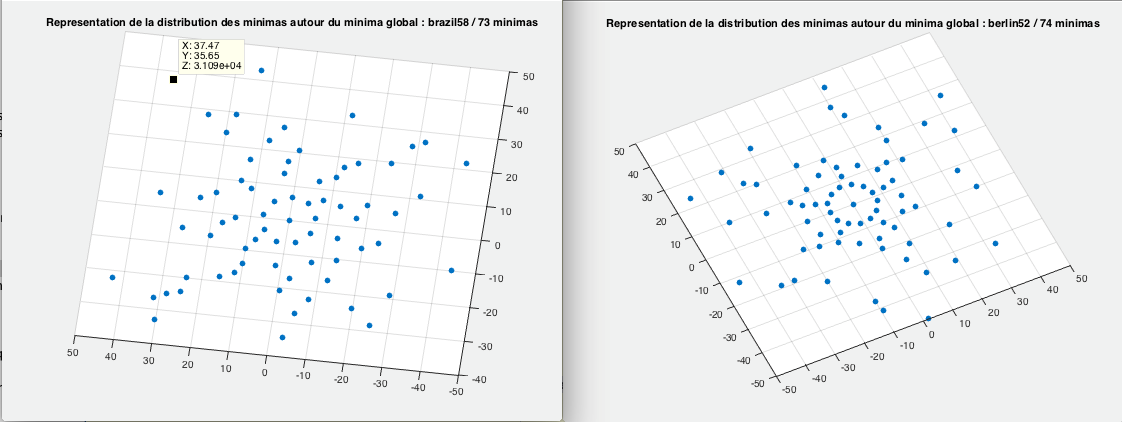
\includegraphics[scale=0.3]{cartes.png} 
\caption{Cartographie des minima locaux sur le benchmark brazil58}
\end{center}
\end{figure}


      Le lieu où la densité des minima nous intéresse est centré sur le minimum global.  On décide alors de comparer la distance des répliques correspondant à des minima locaux au minimum global seul pour diminuer le temps de calcul.
      L’idée est donc d’estimer une distance radiale d’un minimum local au minimum global, sans tenir compte a priori de la distance des minima locaux entre eux. Ainsi, chaque minimum global trouvé peut être placé une carte, on place aléatoirement sur un cercle centré sur le minimum global, de rayon son rapprochement au minimum global.
      L’idée de placer chaque minimum local aléatoirement sur un cercle permet une visualisation en trois dimensions de la densité de minima, et souligne la possibilité d’intégrer une information supplémentaire dans le modèle en jouant sur l’angle aléatoire - par exemple, pour deux minima différents qui ont une distance identique au minimum global, prendre en compte la distance entre eux et en rendre compte dans leur éloignement sur leur cercle.

\section{Recuit Simulé}
\subsection{Principes physiques}
\subsection{Implémentation}

\section{Recuit Quantique}
\subsection{Fonctionement}
\subsection{Classe Routage}

\section{Résultats}


\section*{Conclusion}

\listoffigures
\bibliography{thebibliography}
\end{document}
